\section{Аналитическая часть}

В данном разделе выдвигаются критерии, по которым можно классифицировать методы отображения пользовательского интерфейса.
Проводится краткий обзор существующих методов, а также их классификация согласно выдвинутым критериям сравнения. 
Формализуется постановка задачи в виде IDEF0--диаграммы.


\subsection{Критерии классификации методов отображения интерфейса} 

По результатам опроса, проведенного среди мобильных и frontend--разработчиков, были выявлены критерии, по которым, с точки зрения процесса разработки, можно классифицировать методы создания пользовательского интерфейса:

\begin{itemize}
	\item[---] \textbf{Адаптивность интерфейса}: возможность создания интерфейса, адаптируемого для экранов разного размера или двух ориентаций.
	\item[---] \textbf{Интеграция в существующий код}: возможность постепенного внедрения метода в существующий код или совмещения с другими UI--фреймворками.
	%\item[---] \textbf{Механизм обработки изменений интерфейса}: наличие механизма, позволяющего разработчику не заботиться об отслеживании изменений представлений, порождаемых измением данных, и их отрисовке.
	\item[---] \textbf{Механизм обработки изменений интерфейса}: наличие механизма, посредством которого отслеживаются обновления UI--компонента и инициируется его повторное отображение без участия разработчика.
	\item[---] \textbf{Горячая перезагрузка}: возможность отображать изменения интерфейса, внесенные в код по время исполнения, без перекомпиляции всего приложения. 
\end{itemize}

\subsection{Методы отображения интерфейса в frontend--разработке} 

Frontend --- это визуальная часть веб--сайта, которую пользователь видит и с которой может взаимодействовать при помощи браузера.

Для разработки frontend в качестве базовых инструментов используются следующие языки: 

\begin{itemize}
	\item[---] HTML (от англ. Hypertext Markup Language,  <<язык гипертекстовой разметки>>) --- это система форматирования для отображения материалов, полученных через Интернет \cite{html}. 
	HTML обычно используется для структурирования веб--документа. Он определяет такие элементы, как заголовки или абзацы, и позволяет вставлять изображения, видео и другие медиафайлы.
	\item[---] CSS (от англ. Cascading Style Sheets,  <<каскадные таблицы стилей>>) --- это декларативный язык программирования, используемый для разработки контента веб--сайта \cite{css}. 
	Он определяет то, как HTML--элементы будут выглядеть на веб--странице с точки зрения дизайна, макета на разных устройствах с разными размерами экрана. 
	CSS управляет макетом множества различных веб--страниц одновременно.
	\item[---] JavaScript --- язык программирования, который позволяет создавать сложные функции и интерактивность на веб--сайтах и в веб--приложениях, а также в других вариантах использования, повышает общую интерактивность сайта \cite{js}. 
	Веб--страницы, разработанные с помощью JavaScript, реагируют на действия пользователей и обновляются динамически. %Благодаря JavaScript этот процесс не требует перезагрузки страниц, чтобы отобразить изменения.
\end{itemize}

Использование JavaScript в разработке стало повсеместным: до 97\% веб--сайтов сегодня написаны с его использованием, по сравнению с 88\% десять лет назад. 
За тот же период времени произошли изменения в том, как используется JavaScript: если десять лет назад до 60\% веб--сайтов использовали JavaScript без помощи каких--либо библиотек или фреймворков, то сегодня это делают менее 20\% \cite{сomparison}.
Интерфейсные фреймворки --- это предварительно написанный набор стандартизированного кода HTML, CSS и JavaScript, который разработчики могут использовать для более эффективного создания веб--приложений.
Многие из подобных библиотек --- библиотеки с открытым исходным кодом. По данным с GitHub \cite{github}, самыми популярными являются следующие фреймворки:

\begin{itemize}
	
	\item[---] React --- 221 тысяча Звезд на GitHub \cite{react-github}.
	\item[---] Vue ---  207 тысяч Звезд на GitHub \cite{vue-github}.
	\item[---] Angular --- 94,3 тысячи Звезд на GitHub \cite{angular-github}.
\end{itemize}
  
Рассмотрим каждый из фреймворков детальнее и классифицируем их согласно выделенным критериям.


\subsubsection{React} 

React --- это библиотека JavaScript для создания пользовательских интерфейсов \cite{react}. 
Библиотека была создана для использования в крупных проектах, разрабатывающих объемные интерфейсы и оперирующих данными, которые меняются с течением времени \cite{react-doc}.

Большинство современных frontend--фреймворков используют для управления интерфейсом DOM (от англ. Document Object Model) --- специальную древовидную структуру, которая позволяет управлять HTML--разметкой JavaScript--кода. Управление обычно состоит из добавления и удаления элементов, изменения их стилей и содержимого \cite{real-dom}. 
Основной особенностью библиотеки React является наличие виртуального DOM: это концепция, при которой виртуальное представление пользовательского интерфейса хранится в памяти, синхронизированной с <<реальным>> DOM, React использует его для эффективного обновления пользовательского интерфейса и управления изменениями, вносимыми в него. 
Причина повышенной производительности заключаестся в объеме изменяемой информации: сравнивается элемент и его дочерние элементы с предыдущими и применяются только обновления DOM, необходимые для преобразования в желаемое состояние.

Немаловажной особенностью библиотекм является компонентная архитектура React, которая позволяет разработчикам создавать повторно используемые UI--элементы и размещать их для создания адаптируемых для разных размеров экранов пользовательских интерфейсов.
Концептуально компоненты похожи на функции JavaScript. Они принимают произвольные входные данные (называемые <<props>> или свойствами) и возвращают React--элементы, описывающие, что должно появиться на экране \cite{react-doc}.
Возможность многократного использования компонентов повышает масштабируемость.

Поскольку приложения React используют JavaScript и JSX, разработчики могут применять традиционные методы организации кода. 
JSX преобразуется из XML--подобного синтаксиса, с которым многие знакомы, в JavaScript, необходимый React.
Самое простое объяснение того, как JSX способен использовать XML--подобный синтаксис и преобразовывать его в JavaScript, который используется для генерации элементов React и компонентов, заключается в том, что он просто сканирует XML--подобную структуру и заменяет теги на функции, необходимые в JavaScript \cite{react-book}.
После компиляции выражения JSX становятся обычными вызовами функций JavaScript и вычисляются в объекты JavaScript \cite{react-doc}.

React позволяет внедрять веб--интерфейсы в уже существующий код, например, написанный на JavaScript, без необходимости использования JSX или специальных сборщиков кода. 
То есть можно создавать элементы React прямо в JavaScript.
Для этого используется функция React.createElement(), а компоненты определяются как функции или классы. 
Затем элементы отображаются на странице с помощью ReactDOM.render() \cite{react-doc}.
Такой подход обеспечивает гибкость и возможность интеграции React в существующий код, что может быть полезно при постепенном переходе к использованию React.

Еще одна особенность React – это горячая перезагрузка (Hot Module Replacement - HMR) \cite{hmr}. 
Эта функциональность автоматически обновляет приложение в браузере при сохранении изменений в исходном коде. 
Она позволяет разработчикам быстро увидеть результаты произведенных изменений без необходимости перезагрузки страницы.
Для реализации горячей перезагрузки React использует встроенную функциональность модулей JavaScript. 
При изменении исходного кода React обновляет только те компоненты, которые изменились, не требуя повторной загрузки всего приложения.
Однако горячая перезагрузка --- это функциональность, которая обычно реализуется с помощью сторонних инструментов и плагинов.


\subsubsection{Vue.js}

Vue --- это прогрессивный фреймворк для создания пользовательских интерфейсов \cite{vue}. 

Создатели заявляют, что основной особенность Vue.js, в отличие от других монолитных фреймворков, является возможность постепенного внедрения. 
Библиотеку легко сочетать с другими методами верстки или интегрировать в существующие проекты \cite{vue}.
Также можно использовать Vue.js для управления только частью страницы или функциональности, не переписывая полностью существующий код.
Для внедрения требуется настроить сборку проекта, чтобы поддерживать Vue компоненты и использовать Vue CLI \cite{vue-cli} для управления проектом.

Компоненты в Vue.js являются основным строительным блоком при разработке приложений. 
Они позволяют создавать переиспользуемые и модульные элементы интерфейса, адаптируемые для разных размеров экранов.
Каждый компонент в фреймворке представляет собой независимую единицу, которая содержит свою логику, шаблон и стили.

Vue.js, заимствуя технологию у React, также использует виртуальный DOM, дабы дать разработчику возможность программно создавать, проверять и компоновать нужные структуры пользовательского интерфейса декларативным способом, оставляя прямое управление DOM на усмотрение рендеринга \cite{vue-render}.
В силу реактивного подхода фреймворк использует специальные Proxy--объекты \cite{vue-proxy}. Они содержат в себе другие объекты или функции, позволяющие <<перехватывать>> изменения в них, чтобы узнавать, когда данные стали иными.
После первой отрисовки у компонента будет список отслеживаемых зависимостей, полученных из свойств, затронутых в момент отрисовки. 
Компонент подписывается на каждое из этих свойств.
Когда Proxy перехватывает операцию обновления, все подписанные на свойство компоненты будут уведомлены и перерисованы.

Горячая перезагрузка в Vue --- это функция, которая позволяет заменить экземпляры компонента без перезагрузки страницы. 
При этом сохраняется текущее состояние приложения и заменяемых компонентов.
При создании проекта с помощью Vue CLI --- полноценной системы для быстрой разработки на Vue.js \cite{vue-cli} --- горячая перезагрузка включена по умолчанию. 


\subsubsection{Angular}

Angular --- веб--фреймворк, который позволяет разработчикам создавать быстрые и надежные приложения, предоставляет широкий набор инструментов, API и библиотек для упрощения процесса разработки \cite{angular}. 

Чтобы связывать данные приложения и отображение,  Angular использует HTML--подобный синтаксис для своих шаблонов и компилирует эти шаблоны в набор инструкций, которые создают браузерные DOM--элементы. 
Angular не использует виртуальный DOM, чтобы хранить дерево компонентов в памяти \cite{angular-dom}.
Вместо этого фреймворк предлагает две стратегии для обнаружения изменений: default и onPush \cite{angular-strategy}.
Первая стратегия сводится к рекурсивному проходу по дереву компонентов и сравнению текущего значение с предыдущим для каждого выражения, используемого в шаблоне. 
Если значения отличаются, то фреймворк отмечает их специальным образом и по окончании прохода меняет отображение в DOM.
Стратегия очень удобна, так как разработчику ничего не нужно проверять самостоятельно, однако в больших приложениях может вызывать проблему с производительностью из--за частых перезапусков проверок на любое возникающее событие. 
В борьбе за производительность создатели Angular разработали вторую стратегию --- onPush, которая отключает автоматическое обнаружение изменений.
Тем не менее обнаружение изменений все еще может быть вызвано явно, например, путем вызова соответствующих ассинхронных функций.
Стратегии обновления могут использоваться одновременно: onPush чаще применяют для оптимизации высоконагруженных частей приложения.

Компоненты Angular обеспечивают структуру для организации проекта и деление на простые для понимания части с четкими обязанностями, чтобы код был масштабируемым \cite{angular-components}.
Как React и Vue.js, фреймворк позволяет создавать адаптируемые для разных размеров устройств интерфейсы.

В Angular также есть поддержка горячей перезагрузки (Hot Module Replacement --- HMR) \cite{angular-hmr}. 
Горячая перезагрузка позволяет обновлять только те части приложения, которые были изменены, без полной перезагрузки страницы. 
Это ускоряет процесс разработки и упрощает работу с приложением.
Angular CLI, инструмент командной строки для разработки приложений, поддерживает горячую перезагрузку по умолчанию.

Фреймворк предоставляет возможность постепенного внедрения, что позволяет добавлять Angular--компоненты, модули и функциональность к существующему веб--приложению по мере необходимости.


\subsection{Методы отображения интерфейса в мобильной разработке} 

Двумя самыми популярными в мире операционными системами для мобильных устройств являются Android и iOS \cite{mob-os-stat}. 
Android разработан компанией Google и используется на широком спектре устройств от разных производителей, таких как Samsung, Huawei, Xiaomi и другие \cite{android}.
iOS, в свою очередь, разработана компанией Apple и используется на устройствах iPhone, iPad и iPod Touch \cite{ios}. 

Обе операционные системы имеют свои особенности, интерфейсы и набор функций, и разработчики мобильных приложений часто создают версии своих приложений как для iOS, так и для Android, чтобы охватить более широкую аудиторию пользователей. 
В связи с чем появилось два подхода к разработке программного обеспечения для мобильных устройств: нативная и кроссплатформенная разработка. 

Нативная разработка --- это процесс создания приложений для определенной операционной системы или платформы с использованием языков программирования и инструментов, специфичных для данной платформы \cite{native-crossplatform}. 
Для iOS приложений используется язык программирования Swift или Objective--C, а для Android --- Java или Kotlin.

Кроссплатформенная разработка подразумевает создание приложений, которые могут работать на различных операционных системах без необходимости создания отдельных версий для каждой из них \cite{native-crossplatform}. 
Для кроссплатформенной разработки часто используются фреймворки и инструменты, которые позволяют написать код один раз и запускать его на разных платформах. 
Кроссплатформенная разработка обычно упрощает процесс создания приложений для разных платформ, но может иметь ограничения по производительности и доступу к специфическим функциям устройств.

Далее будут рассмотрены и классифицированы методы отображения интерфейса для каждого из подходов.

\subsubsection{Кроссплатформенная разработка} 

Одними из самых популярных кроссплатформенных мобильных фреймворков являются Flutter и React Native \cite{crossplatform-stat}.

\subparagraph{Flutter}   
\subparagraph{}  

Flutter --- это инструментарий пользовательского интерфейса Google для создания приложений для мобильных устройств, веб--приложений и настольных компьютеров на основе единой кодовой базы \cite{flutter}. 

В силу этой особенности, главным свойством фреймворка является возможность создавать интерфейс, адаптируемый не только для разных размеров конкретного устройства, например, экрана компьютера, а разных типов устройств. 
В связи с этим Flutter обладает большим количеством виджетов и технологий, упрощающих задачу компоновки. 

Официальная документация фреймворка гласит: <<Иногда нецелесообразно переписывать всё приложение на Flutter сразу. 
В таких ситуациях Flutter можно интегрировать в ваше существующее приложение по частям, в виде библиотеки или модуля. 
Затем этот модуль можно импортировать в приложение для Android или iOS, чтобы отобразить часть пользовательского интерфейса вашего приложения во Flutter>> \cite{flutter-integr}.

Виджеты в Flutter представляют собой элементы пользовательского интерфейса, которые позволяют отображать содержимое и взаимодействовать с пользователем. 
Виджеты могут быть простыми, а могут и содержать другие виджеты внутри себя. 
При изменении состояния виджета перестраивается его описание, которое фреймворк сравнивает с предыдущим описанием, чтобы определить минимальные изменения, необходимые в базовом дереве рендеринга для перехода из одного состояния в следующее \cite{flutter-ui}.

Flutter поддерживает функцию горячей перезагрузки, что помогает сократить время создания пользовательских интерфейсов.
Технология работает путем внедрения обновленных файлов исходного кода в работающую виртуальную машину, на которой развернуто приложение. 
После того, как виртуальная машина обновляет классы новыми версиями полей и функций, платформа автоматически перестраивает дерево виджетов, позволяя быстро просмотреть последствия изменений \cite{flutter-hot-reload}.

\subparagraph{React Native} 
\subparagraph{}  

React Native --- это фреймворк с открытым исходным кодом для создания приложений для Android и iOS, использующий React и собственные возможности платформы приложений \cite{react-components}

Особенностью React Native, как кроссплатформенного фреймворка, является наличие возможности создания версий компонентов, зависящих от платформы, чтобы одна кодовая база могла совместно использовать код на разных платформах. С React Native одна команда может поддерживать несколько платформ и использовать общую технологию — React.
Таким образом фреймворк позволяет создавать интерфейс, для разных размеров и ориентаций устройств.

React Native подходит для добавления кода в существующие приложения. 
Выполнив несколько шагов, можно добавить новые функции, экраны, представления на основе React Native и т.д.
Однако, настройка интеграции может отличаться для разных платформ \cite{react-native-integr}. 

При разработке для Android представления создаются с помощью кода на Kotlin или Java, для iOS --- с помощью Swift или Objective-C. 
React Native может вызывать эти представления с помощью JavaScript, используя компоненты React. 
Во время выполнения React Native создает соответствующие представления Android и iOS для этих компонентов. 
Поскольку компоненты React Native поддерживаются теми же представлениями, что и Android и iOS, приложения React Native выглядят и работают так же, как и приложения, созданные с помощью нативных языков. 

Как и виртуальный DOM в React, React Native создает древовидную иерархию для определения представлений.
Когда фреймворк отправляет команды для рендеринга макета, группа теневых узлов собирается для построения теневого (виртуального) дерева, которое представляет изменяемую сторону макета, написанную на соответствующем нативном языке \cite{react-native-render}. 
Затем преобразуется в фактические представления на экране, с помощью Yoga --- кроссплатформенного движка верстки \cite{yoga}.

Также как и React, React поддерживает функцию горячей перезагрузки.
\subparagraph{}  
\subsubsection{Нативная разработка Android} 

\subparagraph{Метод с использованием XML} 
\subparagraph{}  
Классический метод верстки на Android предполагает размещение элементов на экране с помощью XML--файла \cite{xml-android}.
XML --- это расширяемый язык разметки, который предоставляет правила для определения любых данных.
XML--файл состоит из различных тегов и атрибутов, которые задают верстку всему экрану. 
В среде разработки, благодаря использованию специальных инструментов, можно наблюдать, как будет выглядеть макет на различных типах и форматах дисплеев.

Сам по себе XML--файл представляет только разметку, то есть то, как элементы интерфейса будут выглядеть и располагаться на экране. 
Для управление логикой работы экрана необходимо использовать дополнительный код на языке Java или Kotlin.
Аналогом виртуального DOM в XML--верстке на Android можно считать View hierarchy, которая представляет собой иерархию всех пользовательских интерфейсных элементов (View) в XML--файлах \cite{dom-android}. 
Используя XML для верстки интерфейса на Android, разработчики создают дерево View элементов, которое затем обрабатывается и отображается на экране устройства. 
При обновлении интерфейса в приложении система Android перестраивает и обновляет View hierarchy по аналогии с тем, как виртуальный DOM обновляет DOM веб-приложений. 
Таким образом при XML--верстке на Android присутствует механизм автоматического обновления UI--компонентов при изменениях, которые позволяют повторно отобразить интерфейс без необходимости вмешательства разработчика.

XML--верстка хорошо интегрируется в существующий код, позволяя постепенно внедрять новые методы в существующую структуру приложения и сочетаться с другими UI--фреймворками.

Метод не поддерживает горячую перезагрузку, что означает, что для просмотра изменений, внесенных в код во время исполнения, требуется перезапуск приложения.

\subparagraph{Jetpack Compose} 
\subparagraph{}  
Jetpack Compose --- это современный инструментарий для создания собственного пользовательского интерфейса Android \cite{jetpack}.

Как декларативный инструментарий пользовательского интерфейса, Jetpack Compose хорошо подходит для разработки и реализации макетов, которые настраиваются для отображения контента по--разному в различных размерах \cite{jetpack-layout}.

Jetpack Compose позволяет поэтапно внедрять свой метод создания UI в существующий код приложения, постепенно заменяя старые View--based компоненты новыми Compose--компонентами \cite{jetpack-layout}. 
Также возможна параллельная работа с другими UI--фреймворками.

С помощью Compose можно создать свой пользовательский интерфейс, определив набор составных функций, которые принимают данные и генерируют элементы. 
В модели компоновки дерево пользовательского интерфейса создается за один проход. 
Сначала каждому узлу предлагается измерить себя, затем рекурсивно измерить все дочерние узлы, передавая ограничения размера вниз по дереву дочерним узлам. 
Элементы компонуются в синтаксическое дерево, которое представляет структуру пользовательского интерфейса. 
Это дерево называется Composable.
Composables можно вкладывать друг в друга, создавая сложные пользовательские интерфейсы.

В Jetpack Compose существует аналог виртуального DOM, который называется Recomposition \cite{jetpack-lifecycle}. 
Recomposition подходит для пересоздания только тех частей пользовательского интерфейса, которые изменились, вместо пересоздания всего UI. 
Это позволяет эффективно обновлять UI при изменении данных или состояния приложения.
Recomposition в Jetpack Compose работает путем сравнения и обновления Composables, которые используются для отображения пользовательского интерфейса. 
При изменении данных или состояния, Composables, которые зависят от этих изменений, будут пересозданы, а затем сравнены с предыдущими версиями и обновлены на экране.

Одним из недостатков фреймворка Jetpack Compose является отсутствие возможности быстрой перезагрузки кода без перезапуска всего приложения.
Отсутствие функции hot reload делает процесс разработки менее удобным по сравнению с другими фреймворками.
\subparagraph{}  
\subsubsection{Нативная разработка iOS} 

\subparagraph{UIKit} 
\subparagraph{}  
UIKit предоставляет множество функций для создания приложений, включая компоненты, которые можно использовать для создания базовой инфраструктуры приложений для iOS, iPadOS или tvOS \cite{uikit}.

Интерфейс с помощью UIKit можно создавать двумя способами \cite{uikit2}: с использованием Interface Builder --- инструмента, позволяющего разработчикам визуально создавать и настраивать пользовательские интерфейсы --- посредством редактирования «.storyboard» и «.xib» файлов, которые описывают интерфейс с помощью XML (то есть без написания кода), или с помощью Swift или Objective--C программно, например, с помощью frame \cite{uikit-frame} или AutoLayout \cite{uikit-autolayout}. 
Interface Builder не всегда предоставляет возможность создавать интерфейсы, адаптируемые ко всем типам устройств, в отличие от второго метода. 

UIKit легко интегрируется в существующий код, позволяя постепенно внедрять новые методы и компоненты в уже существующую структуру приложения. 
Он также хорошо совмещается с другими UI--фреймворками, такими как SwiftUI \cite{uikit-integr}.

В UIKit Apple каждый экран приложения представлен иерархией view --- объектов класса UIView или его наследников \cite{uikit-uiview}. 
После изменения данных модели, UIKit автоматически обновляет и перерисовывает только те части иерархии, которые фактически изменились, минуя объекты, которые остались неизменными.
Это позволяет обновлять интерфейс более эффективно.

UIKit не поддерживает горячую перезагрузку, поэтому для отображения изменений, внесенных в код во время исполнения, требуется перекомпиляция и перезапуск приложения.
Однако при проектировании интерфейса через Interface Builder появляется возможность визуально создавать элементы экрана.

\subparagraph{SwiftUI} 
\subparagraph{}  

SwiftUI --- это декларативный и модернизированный фреймворк пользовательского интерфейса Apple, который предоставляет нативный способ создания интерфейсов для iOS, macOS, watchOS и tvOS \cite{swiftui}.

SwiftUI поддерживает адаптивную разметку, что позволяет создавать интерфейсы, которые автоматически адаптируются под разные размеры экранов и ориентации. 
Можно использовать специальное UI--элеменеты, например, Stack, а также модификаторы для управления распределением элементов интерфейса на различных устройствах и экранах \cite{swiftui-stack}.

SwiftUI может постепенно внедряться в существующий код приложения, позволяя создавать новые экраны или переписывать существующие компоненты постепенно. 
Он также может быть интегрирован с UIKit, что позволяет использовать оба фреймворка в одном приложении, например, для перехода на SwiftUI постепенно \cite{uikit-integr}.

SwiftUI предлагает декларативный подход к проектированию пользовательского интерфейса и автоматически обновляет затронутые части интерфейса при изменении данных.
Чтобы обновлять представления при изменении данных, классы модели данных необходимо объявить наблюдаемыми объектами (observable) \cite{swiftui-observ}.
Чтобы изменения в данных, получаемые от пользователя, возвращались в модель, элементы управления пользовательского интерфейса связываются со свойствам модели.
Управление состоянием является основой для создания эффективных приложений, которые поддерживают актуальность информации для пользователя.

SwiftUI не поддерживает функцию горячей перезагрузки.
Однако Xcode --- интегрированная среда разработки программного обеспечения для платформ macOS, iOS, iPadOS, watchOS, tvOS --- при создании пользовательского приложения с помощью SwiftUI предоставляет возможность отображать предварительный просмотр содержимого представления, которое остается актуальным по мере внесения изменений в код представления. 
Эта функциональность доступна при использовании в коде специальных макросов \cite{swiftui-preview}.

\subsection{Результаты анализа} 

Классификация методов отображения пользовательского интерфейса приведена в таблице 1. % \ref{table1}. 
Для краткости записи в данной таблице используются следующие обозначения описанных критериев:
 \begin{itemize}[label=---]
	\item К1 --- адаптивность интерфейса;
	\item К2 --- интеграция в существующий код;
	\item К3 --- механизм обработки изменений интерфейса;
	\item К4 --- горячая перезагрузка.
\end{itemize}

\begin{table}[!htb]
	\label{table1}
	\begin{center}
		\caption{Классификация методов отображения пользовательского интерфейса}
		\begin{tabular}{|p{5.5cm}|c|c|c|c|c|c|}
			\hline
			\textbf{Класс метода} & \textbf{Название} & 
			\textbf{К1} & \textbf{К2} & \textbf{К3} & \textbf{К4}\\
			\hline
			{Frontend--разработка} & 
			React & 
			+ & + & + & + \\
			\cline{2-6} & Vue & 
			+ & + & + & + \\
			\cline{2-6} &Angular & 
			+ & + & + & + \\
			\hline
			{Кроссплатформенная  \newline{} мобильная разработка} & 
			Flutter &  
			+ & + & + & + \\
			\cline{2-6} & React Native &  
			+ & + & + & + \\
			\hline
			{Нативная мобильная \newline{} разработка Android} & 
			Метод с использованием XML &  
			+ & + & + & - \\
			\cline{2-6} & Jetpack Compose &  
			+ & + & + & - \\
			\hline
			{Нативная мобильная \newline{} разработка iOS} & 
			UIKit &  
			+ & + & + & - \\
			\cline{2-6} & SwiftUI &  
			+ & + & + & - \\
			\hline
		\end{tabular}	
	\end{center}
\end{table}

\subsection{Постановка задачи}

Этап создания интерфейса является одной из ключевых стадий разработки приложений и веб--сайтов \cite{website}, определяющим успех проекта и уровень его пользовательской привлекательности. 
Существует множество методов отображения пользовательского интерфейса, предоставляющих различные возможности разработки. 
По результатам классификации наиболее популярных из них на первый план выходит отсутствие горячей перезагрузки в ряде фреймворков.
Данная функция экономит время разработки, обновляя только те элементы интерфейса, которые были изменены, без необходимости перезагрузки всего приложения. 
Разрабатываемый метод должен предоставлять возможность динамически отображать изменения пользовательского интерфейса.

XML --- язык форматирования документов \cite{xml}, основан на тегах, которые определяют начало и конец элементов данных.
Каждый XML---документ начинается с корневого элемента, содержащего все остальные. 
Элементы могут содержать атрибуты, которые дополняют информацию о содержимом. 
XML позволяет создавать иерархические структуры данных.
Интерфейс должен задаваться посредством написания XML--файла, а разрабатываемый метод должен предоставлять возможность отображать изменения интерфейса на основе обработки этого файла.

Задача формализована с помощью диаграммы IDEF0 уровня A0, представленной на рисунке  \ref{fig:idef0}.

\begin{figure}[!htb]
	\centering
	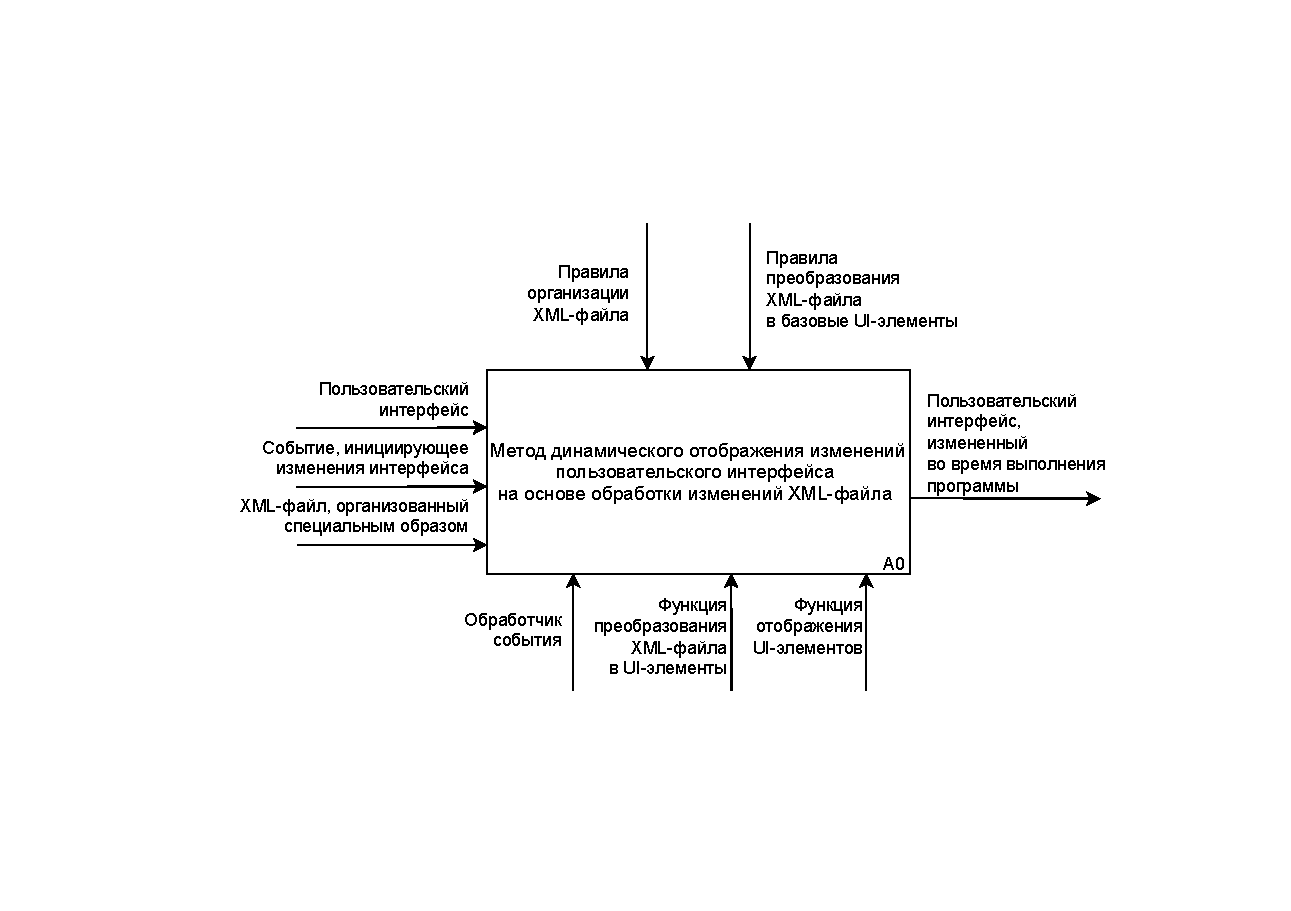
\includegraphics[scale=1]{img/A0.pdf}
	\caption{IDEF0 --- диаграмма уровня А0}
	\label{fig:idef0}
\end{figure}

\newpage{}
\subsection*{Вывод}

В данном разделе были выдвинуты критерии классифицикации методов отображения пользовательского интерфейса.
Проведен краткий обзор существующих методов, а также их классификация согласно выдвинутым критериям сравнения. 
Была формализована постановка задачи.

\pagebreak
